\begin{figure}
\begin{boxedminipage}{0.495\hsize}
\begin{lstlisting}[language=LMR,basicstyle=\lstfigurestyle,breaklines=true,frame=none]
def f$_1$ =
  fix f$_2$ {
    fun n$_3$ {
      ifz n$_4$ then 1
      else n$_5$*f$_6$(n$_7$-1)
    }
  }
def n$_8$ = f$_9$ 5
\end{lstlisting}
\end{boxedminipage}\hfill
\begin{boxedminipage}{0.495\hsize}
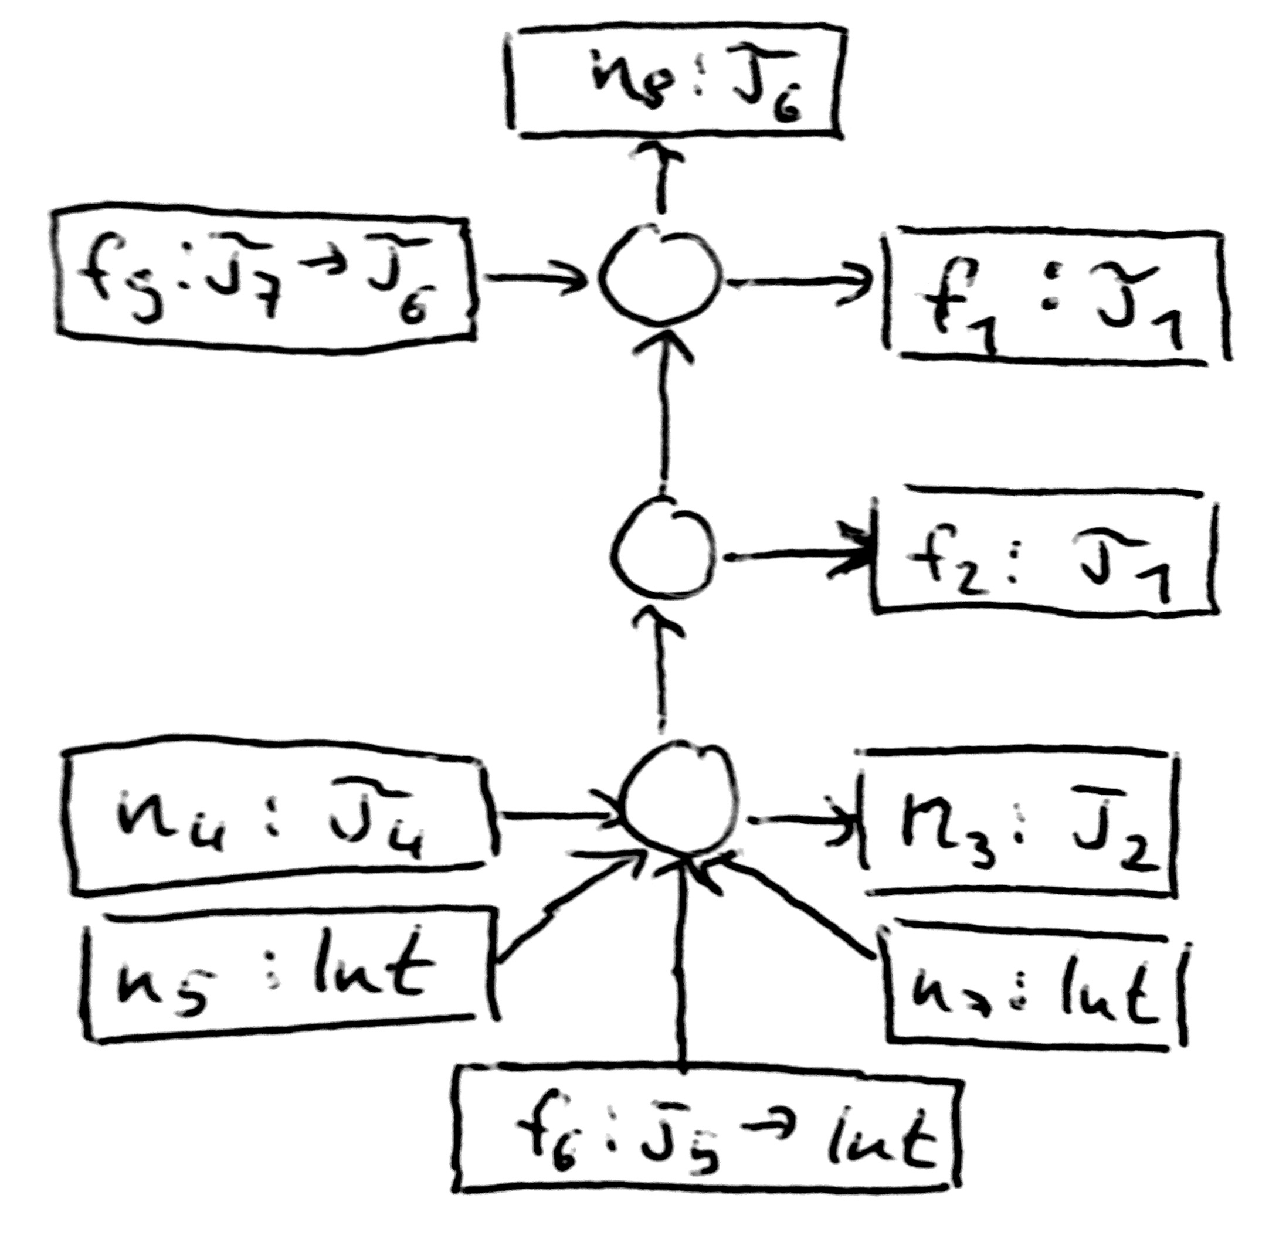
\includegraphics[width=\hsize]{figures/infgraph.pdf}
\end{boxedminipage}
\begin{boxedminipage}{0.495\hsize}
\small
\center{type constraints}
\[
\begin{array}{l}
\ceq{\vty{2} \rightarrow \vty{3}}{\vty{1}}\\
\ceq{\vty{4}}{\usebox{\boxint}}\\
\ceq{\usebox{\boxint}}{\vty{3}}\\
\ceq{\usebox{\boxint}}{\vty{5}}\\
\end{array}
\]
\vfill
\end{boxedminipage}\hfill
\begin{boxedminipage}{0.495\hsize}
\small
\center{solutions to constraints}
\[
\begin{array}{l}
\ceq{\vty{1}}{\usebox{\boxint} \rightarrow \usebox{\boxint}}\\
\ceq{\vty{2}}{\usebox{\boxint}}\\
\ceq{\vty{3}}{\usebox{\boxint}}\\
\ceq{\vty{4}}{\usebox{\boxint}}\\
\ceq{\vty{5}}{\usebox{\boxint}}
\end{array}
\]
\end{boxedminipage}

\label{fig:inference}
\caption{Type inference.}
\end{figure}
